\documentclass[a3paper]{article}
\usepackage{graphicx} 
\usepackage[utf8]{inputenc} % Кодировка документа
\usepackage[T2A]{fontenc} % Внутренняя кодировка шрифтов
\usepackage[russian]{babel} % Поддержка русского языка
\usepackage{pdflscape} % Для альбомной ориентации
\usepackage[left=2cm,right=2cm,top=2cm,bottom=2cm]{geometry} % Задаем отступы
\pagestyle{empty} % Удаляем номера страниц
\usepackage{hyperref}

\begin{document}
	\begin{landscape}
		\setcounter{figure}{2}
		\begin{figure}[h]
		\centering
		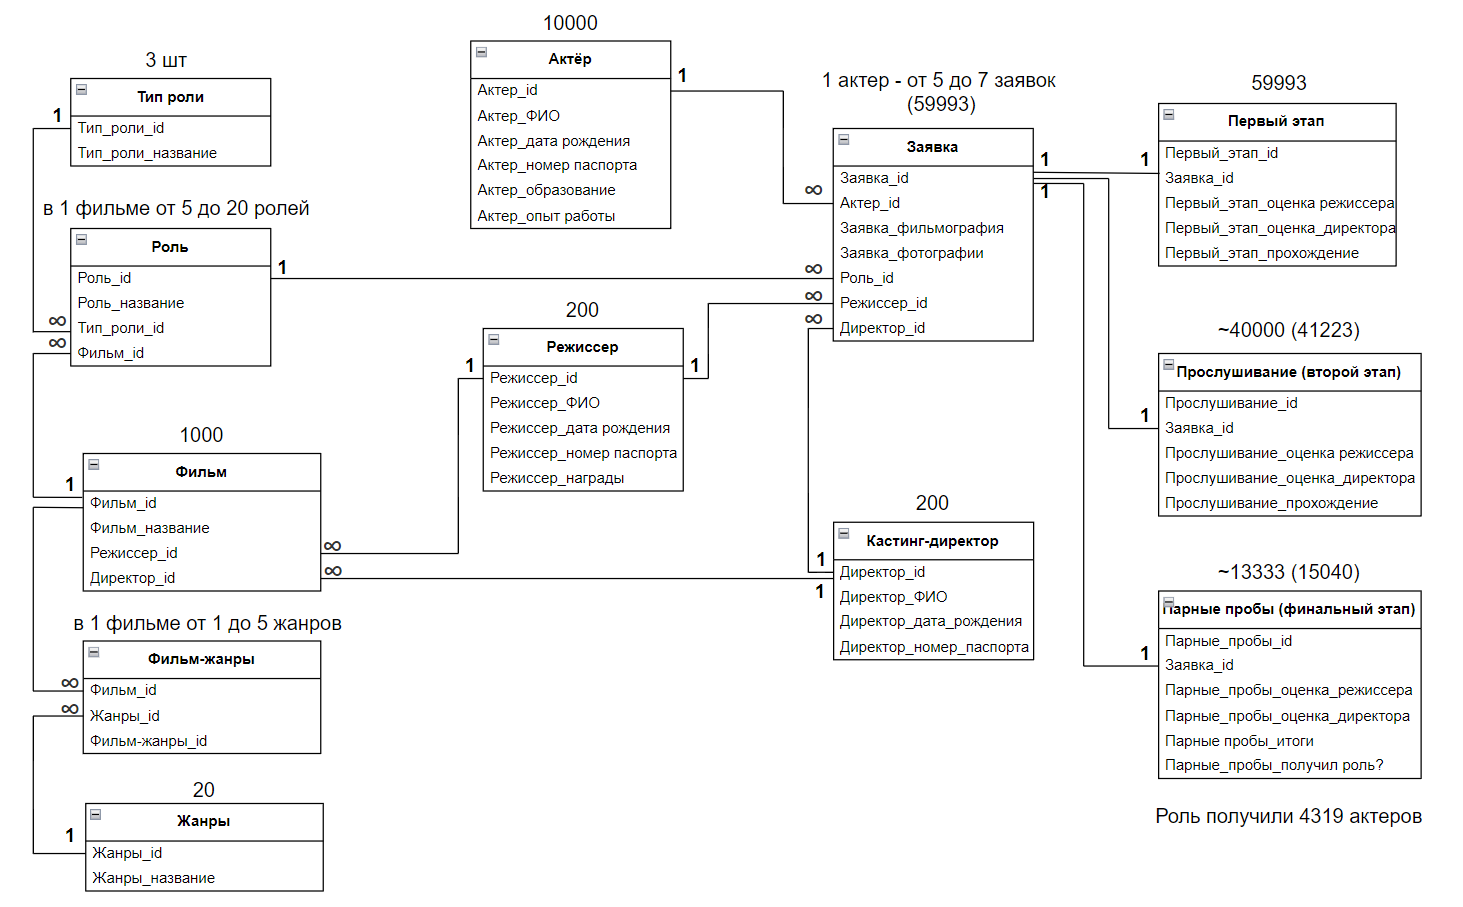
\includegraphics[width=1.0\linewidth]{dataBase.png}
		\caption{Схема базы данных}
		\label{fig:dataBase}
	\end{figure}
	
	\newpage
	
	\begin{figure}[h]
		\centering
		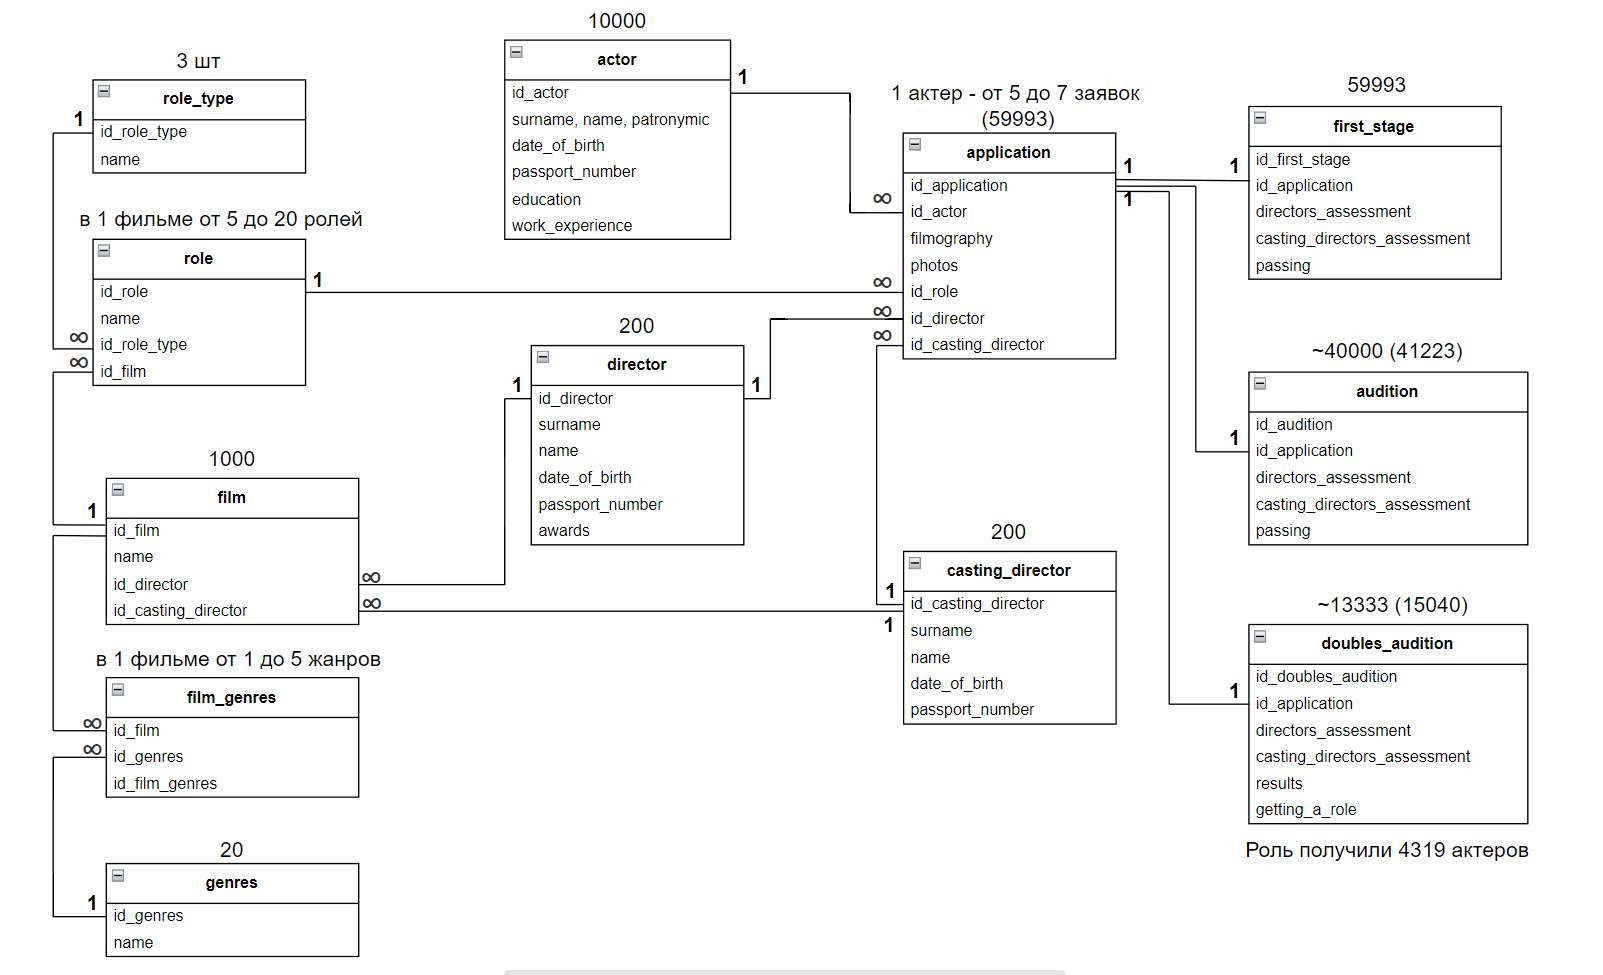
\includegraphics[width=1.0\linewidth]{ENG_database.png}
		\caption{Database schema}
		\label{fig:dataBase}
	\end{figure}
    
	\end{landscape}    
\end{document}